\chapter{Développement}

  Le développement du programme s’est fait en plusieurs étapes clef.

  Dans un premier temps nous avons créé les différentes classes prévues dans notre diagramme de classes UML. Ce qui implique l’écriture des headers et également des constructeurs de base tels que nous les concevions à ce moment. Nous nous sommes chargés ensuite de mettre en place l’initialisation des planètes sur la grille du monde, pour cela nous nous sommes occupés de terminer le constructeur de l’objet world (qui n’a presque pas changé depuis). Enfin nous avons implémenté les méthodes dont nous étions sûrs de leur nécessité comme les getters et les setters de certains champs critiques, ainsi que des convertisseurs, puisque nous savions que les objets (agents) présents dans notre grille monde allaient devoir être supprimés puis remplacés à la volée durant la simulation. Par exemple nous avons créé une méthode permettant de « convertir » un objet free planet en un objet colonized planet en ne prenant en paramètre que des champs critiques. Dans ce cas précis, nous donnons en paramètre une référence vers la faction de la nouvelle planète colonisée. C’est également dans cette partie que nous avons créé la fonction scheduler qui parcourt les agents vivants et les fait agir. Cette partie que l’on pourrait qualifier de mise en place du système a duré pendant environ 20\% du projet.

  Après cette partie mise en place des agents dans la simulation, nous nous sommes attaqués aux méthodes run(), c’est-à-dire aux actions propres des agents dans la simulation que nous venions de mettre en place. Nous nous sommes donc d’abord chargés de la méthode run des planètes colonisées puisque c’est la plus complexe. Nous avons réalisé à ce moment-là que des méthodes run sur toutes les planètes n’étaient pas nécessaires, car il n’était pas prévu que les planètes sans faction agissent. Nous avons alors pu lancer nos premières simulations. Celles-ci nous ont révélé des erreurs non prévues, comme lors de la fin de la simulation qui renvoyait une segmentation fault à la suppression de la faction. S’en suivit donc une phase de bug fixing.

  C’est notamment à ce moment-là que nous avons décidé de donner aux objets free planet une faction neutre pour avoir accès à plus de données. Comme celle-ci ne pouvait être créée qu’une seule fois (puisque en tant que faction fantôme, elle n’est pas un agent) nous avons décidé d’en faire un singleton. L’implémentation en elle-même des méthodes run() pour définir les actions des agents n’a duré que 5\% du temps du projet mais la partie bug fixing a dû durer elle 60\% du temps. En effet nous avons notamment rencontré des difficultés lors des conversions durant la simulation. Celles-ci rendaient les références des planètes voisines obsolètes. Cette mise à jour du voisinage fut la principale cause d’erreur durant le TP.

  Enfin, une fois une version stable obtenue, et des simulations concluantes nous nous sommes lancés dans la création d’une interface en Qt avec un afficheur d’images à la place des caractères ASCII afin de découvrir les possibilités de l’outil. Pour ce faire nous avons utilisé très simplement l’outil en affichant des cercles pour chaque planète de couleur différente suivant la faction. Cette fonction display est appelée après chaque appel au scheduler. Nous avons également ajouté un tableau affichant les statistiques de chaque agent faction afin de voir en temps réel leur évolution. Nous avons ensuite peaufiné cet afficheur en rajoutant des images et des valeurs pour chaque planète (son économie et sa défense). Pour optimiser l’afficheur nous avons rajouté un booléen (qui n’était pas prévu à la base) sur les agents planètes déterminant si elle avait changé depuis le dernier tour (si ses valeurs ont évolué) et de ce fait si son affichage doit être mis à jour. Ce booléen est vrai à la construction des agents, ce qui fait que tout nouvel agent doit être affiché. De plus le getter de ce booléen passe automatiquement celui-ci à false en fin de traitement, de manière qu’une fois l’affichage mis à jour, celui-ci ne soit plus effectué tant que la méthode changed() (qui passe le booléen à true) n’a pas été appelée. Cette partie nous a permis de découvrir une erreur de référence concernant les factions puisque les valeurs affichées par le tableau étaient totalement erronées ce qui faussait également la simulation. Cette partie a duré 10\% du temps du projet.

  Pour terminer nous nous sommes chargés de modifier les valeurs de nos simulations afin de les rendre plus pertinentes. Nous avons également rajouté des constantes statiques dans nos classes permettant de contrôler plus efficacement les paramètres de notre simulation. Par exemple nous avons créé une constante \cppinline{MAX_COLONY_DEFENSE} qui définit la valeur max de défense que peut avoir une planète. Enfin nous avons terminé le développement du projet par une phase de bug fixing qui nous a notamment permis de corriger des problèmes de fuite mémoire (à l’aide de valgrind). Nos agents planètes envoyant des demandes de subvention aux agents factions, ces demandes lors de leur traitement n’étaient pas supprimées ensuite, ce qui impliquait qu’au fur et à mesure des simulations, les factions perdaient inutilement de l’argent.

  \section{Patrons de conception}

  Durant le TP, 3 patrons de conception notables ont été utilisés:
  
  \subsection{Patron composite}
  \begin{center}
    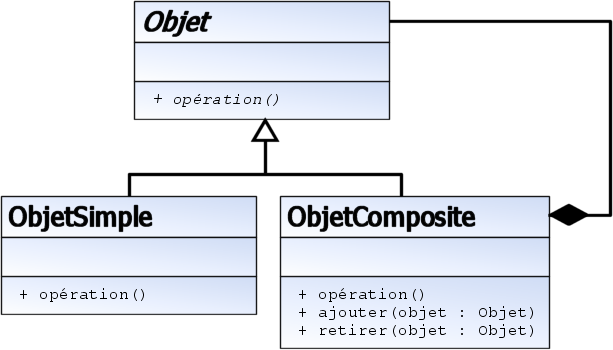
\includegraphics[height=4cm]{images/composite.png}
  \end{center}

  Dans notre code chaque agent planète a connaissance de ses voisins, sachant que ses voisins peuvent être soit des planètes libres, soit des planètes colonisées. Dans le code ce patron apparaît ainsi:

  \begin{cppcode*}{gobble=4}
    class Virtual_planet
    {protected:
      std::vector<Virtual_planet* > neighbourhood_;
    };
  \end{cppcode*}
  Ce patron nous évite bien sur de complexifier le code avec un classe voisin qui alourdirait grandement nos simulations.

  \subsection{Patron stratégie}
  \begin{center}
    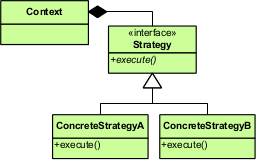
\includegraphics[height=4cm]{images/strategy.png}
  \end{center}

  Nous devons dans notre simulation traiter différemment nos agents en fonction de leur type, mais ceux ci doivent être stockés sur une même grille monde. De ce fait nous avons été obligés de recourir au patron stratégie. Dans le code, celui-ci apparaît de la manière suivante:

  \begin{cppcode*}{gobble=4}
    bool Free_planet::is_attacked(Virtual_planet *) {
      bool res = true;
        if(world_.gen_mt(0,4)==0){ //Une chance sur 5 de ne pas réussir
          res=false;
      }
      return res;
    }

    bool Colonized_planet::is_attacked(Virtual_planet *attacker) {
      bool res = true;
      if (attacker->get_faction() == this->get_faction()) {
          res = false;
      }
     
        if (colony_defense_ > world_.gen_mt(0,99)){ //plus la defense est grande, plus les chances de conquete sont reduite (defense <=50)
          res = false;
          colony_defense_ -= world_.gen_mt(1,25); //la defense et l'eco baisse a cause de l'assaut
          colony_production_ -= world_.gen_mt(1,25);
          change();
        }
      //On supprime l'agent de la liste d'attente puiqu'il va etre elimine ainsi que de sa faction
      if (res == true) {
          world_.remove_waiting_agent(this);
          faction_.remove_colony(this);
          faction_.remove_demand(this);
      }
      return res;
    }
  \end{cppcode*}
  Ce patron nous permet donc pour une même instruction, d’obtenir un comportement différent en fonction de l’agent activé.

  \subsection{Singleton}

  \begin{center}
    
\includegraphics[height=3cm]{images/single.png}
  \end{center}

  Comme expliqué précédemment nous avons décidé de rajouter une faction neutre à notre code mais celle-ci ne devait pas peser dans la mémoire de nos simulations. Nous en avons donc fait un singleton:
  \begin{cppcode*}{gobble=4}
    class Neutral_faction: public Faction
    {
    private:
      static Neutral_faction* instance_;
      Neutral_faction(World& world);
    public:
      static Neutral_faction* get_instance(World& world);
      static void dispose();
    };
  \end{cppcode*}

  Il est à noter que pour terminer proprement le programme il faut appeler la méthode dispose() de ce singleton qui supprime proprement l’instance car le C++ ne vide pas automatiquement celle ci à la fin du programme.

  \section{Présentation des interfaces}

  Nous avons développé deux interfaces durant notre projet, la première en ASCII, qui nous a notamment permis de debugger le programme. Nous avons également implémenté une interface graphique, plus agréable à regarder et plus ergonomique. Cette implémentation nous a permis entre autres d’apprendre les rudiments de Qt.

  \subsection{Interface console}
  L’affichage en mode console est une méthode de l’objet monde. Elle affiche dans la sortie standard chaque case de la grille du monde ainsi que les statistiques des factions. Son code est le suivant:

  \begin{cppcode*}{gobble=4}
    void World::display() {
      for (unsigned i = 0; i < len() +2; i++) cout << "-";
    cout << endl;
      cout << "x|";
      for (unsigned i = 0; i < len(); i++) cout << /*"|"<<*/ i%10 <<"|";
    cout << endl;
     
      for (unsigned i = 0;i < hei(); i++) {
          cout <</* "|" <<*/ i%10 << "|";
          for (unsigned j = 0;j < len();j++) {
              cout << get_grid(j,i)->display();
              cout << "|";
          }
          cout << endl;
      }
      for (unsigned i = 0; i < len() +2; i++)
    cout << "-";
      cout << endl <<endl;
     
      cout << "Stats faction:" << endl;
          for(list<Faction>::iterator it = factions_.begin();
    it!=factions_.end();
    it++ ) {
          cout << it->toString();
    }
      cout << endl << endl;
    }
  \end{cppcode*}

  Le principe est simple: on parcourt chaque case de la grille monde et on appelle la méthode display() qui est une fonction surchargée suivant le patron stratégie. Ainsi les factions ont un caractère ASCII représentant leur capitale et un représentant leurs colonies. Si on appelle la méthode display() sur une colonie le caractère correspondant sera donné etc. Si la planète est libre la méthode renverra un simple point.
  A l’écran cette interface apparaît ainsi:

  \begin{center}
    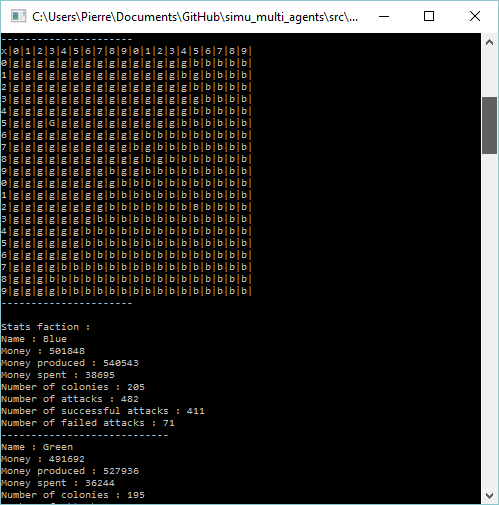
\includegraphics[height=12cm]{images/console.png}
  \end{center}


  \subsection{Interface Graphique}
  L’interface graphique faite sur Qt a pour avantage d’afficher plus de données que l’interface console et ce de manière plus claire. Elle possède elle aussi une fonction display() qui dessine les planètes et leurs statistiques quand celles-ci ont besoin d'être mises à jour (voir partie développement pour savoir comme l’afficheur détermine s’il doit redessiner une planète). L’afficheur graphique également met à jour les informations des factions en temps réel sur la droite de la fenêtre.
  
  Il permet également de distinguer les factions à l’aide d’une couleur et non plus d’un caractère. Ceci est dû au fait que chaque faction possède des champs \cppinline{color_colony} et \cppinline{color_motherland} qui sont les couleurs (\cppinline{string}) à donner aux fonctions de dessin de Qt pour obtenir certaines couleurs. Ainsi la fonction de Qt n’a qu’à appeler la méthode \cppinline{get_color()} (qui est aussi surchargée) sur chaque agent planète et ainsi les couleurs affichées seront celles liées aux factions. Si la planète est libre sa couleur sera par défaut le gris.
  
  Comme vu précédement, un champ \cppinline{change} nous permet de savoir si l’agent doit être redessiné. Si c’est le cas nous devons supprimer d’abord les anciens objets que nous avions dessiné. Pour cela, nous avons créé une classe \cppinline{QPlanet}, composée de pointeurs vers une ellipse, deux images et deux textes, que nous créons et supprimons au besoin. Ainsi nous évitons les fuites mémoire.
  
  A l’écran l’interface apparaît ainsi:
  \begin{center}
    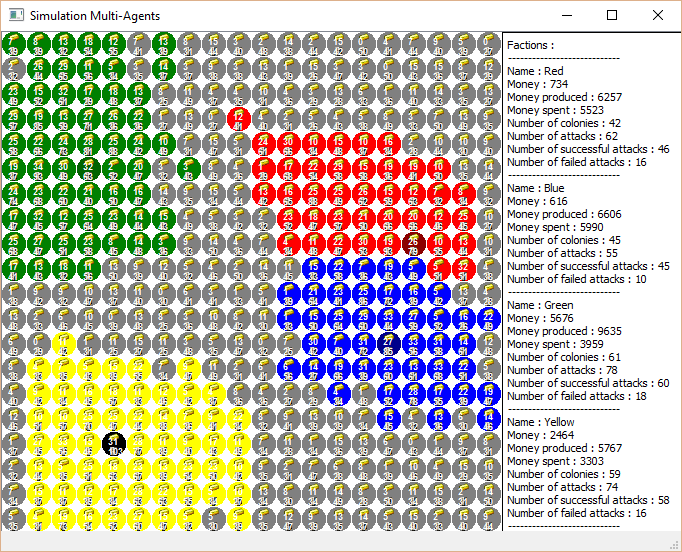
\includegraphics[height=12cm]{images/gui.png}
  \end{center}

  Le désavantage de cette interface est qu’elle ralentit beaucoup la simulation.

  Source des images: \href{https://fr.wikipedia.org}{\texttt{https://fr.wikipedia.org}}
